\textit{This chapter concerns the most important parts about how this project has been implemented. It has been split into several sections.}

\Mathias{Less calculations on the drone, better to move to another computer/cluster with more power than the drone has available from its battery}
\Mathias{Image of camera and drone seen from the side. Show what happens to the drones position estimation when it drifts down/up}
\section{Indoor localization}
\textit{In order to do indoor flying there is a need of some sort of localization since GPS is not available. Vision was decided based on what mostly others are using and some further advantages. Instead of making the vision, it is decided to use an existing tracker called MarkerLocator written by Henrik Midtiby. However the MarkerLocator lacks a proper quality measure so that is implemented. A few tests were made and the MarkerLocator with implemented quality measure suits the needs in this project.}


In order to do accurate flying indoor a localization system is needed. In the Related Work section, it can be seen vision with a camera mounted pointing down is used by others. Compared to use one or more cameras mounted on the drone, an advantage of using a camera mounted on the ceiling is that the camera will not be harmed if the drone crashes and that one camera can be used to detect several drones. However if the position is needed in more than 2D, more than one camera might be needed(depending on the algorithm used) but it still scales better than mounting one or more cameras on each drone. \\

Based on previous experience, the MarkerLocator written by Henrik Midtiby was chosen as indoor localization. Its using OpenCV\footnote{\url{http://opencv.org/}} and implemented in python. It works by detecting markers as shown in figure \ref{fig:markerlocator_marker}
\Mathias{insert image of markerLocator marker with different orders}


\begin{figure}[H]
    \centering
    \begin{subfigure}[b]{0.2\textwidth}
        
\includegraphics[width=\textwidth]{graphics/marker_order_4.pdf}
        \caption{Marker of order 4 used to get the 2D position of a drone}
        \label{fig:markerlocator_order_4}
    \end{subfigure}
    \quad %add desired spacing between images, e. g. ~, \quad, \qquad, \hfill etc. 
      %(or a blank line to force the subfigure onto a new line)
    \begin{subfigure}[b]{0.2\textwidth}
        
\includegraphics[width=\textwidth]{graphics/marker_order_6.pdf}
        \caption{Marker of order 6 used to get the 2D position of a drone}
        \label{fig:markerlocator_order_4}
    \end{subfigure}
    \caption{The markers have one arm less than the order of the marker for the MarkerLocator to detect the orientation of the marker}\label{fig:markerlocator_marker}
\end{figure}




The MarkerLocator works by making a convolution sum of a complex kernel on each frame obtained from the camera.
The location where if fits best is said to be the location of the marker in the frame.
How it works in detail is out the scope of this project.
The markers shown in figure \ref{fig:markerlocator_marker} is of different orders.
The order is equal to the number of black arms minus one since the missing arm is used to detect the orientation of the marker. 
Different orders can be used and thereby detect more than one marker in each frame. Unfortunately it can only get the 2D position and 1D orientation of the marker.
Since doing a convolution of the entire frame is relatively slow \footnote{Processing one fullHD frame takes approximately 0.38 sec. Measured with build in timer in the MarkerLocator}, the MarkerLocator has a mode called WindowMode.
It works by searching in only a small area around the last known position of the marker and thereby speeding up the progress\footnote{Approximately 0.0041 sec}. 

\begin{figure}[H]
    \center
    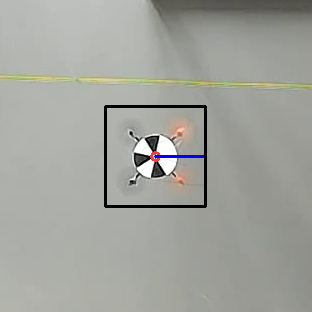
\includegraphics[width=0.4\textwidth]{graphics/markerlocator_window.png}
  	\caption{The MarkerLocator searches only for the marker around the last known position of the marker in a frame of 100*100px.}
    \label{markerlocator_windowmode}
\end{figure}
If the marker moves out of the window, the MarkerLocator is still looking in only that window.
Therefore it is important to have a quality measure that can be used to decide whenever a full convolution of the frame has to be done or if the marker has been found within the window. 

The MarkerLocator has a quality measure build-in used to tell how well the marker is detected. However it is not used in the MarkerLocator to tell if a full convolution has to be done. 
The quality measure implemented in the MarkerLocator is a hack \footnote{Said by Henrik Midtiby} and is known from previous applications that it is a bad measure of the right marker is detected.

In cooperation with Henrik Midtiby a few quality measures was developed. The overall idea was to compare the kernel used to do the convolution with the marker found in the frame.
Different algorithms where used to give a normalized value telling how similar the found marker is to the kernel. Figure \ref{fig:markerlocator_algorithms} shows the different solutions tried.\\

\begin{figure}[H]
    \centering
    \begin{subfigure}[b]{0.3\textwidth}
        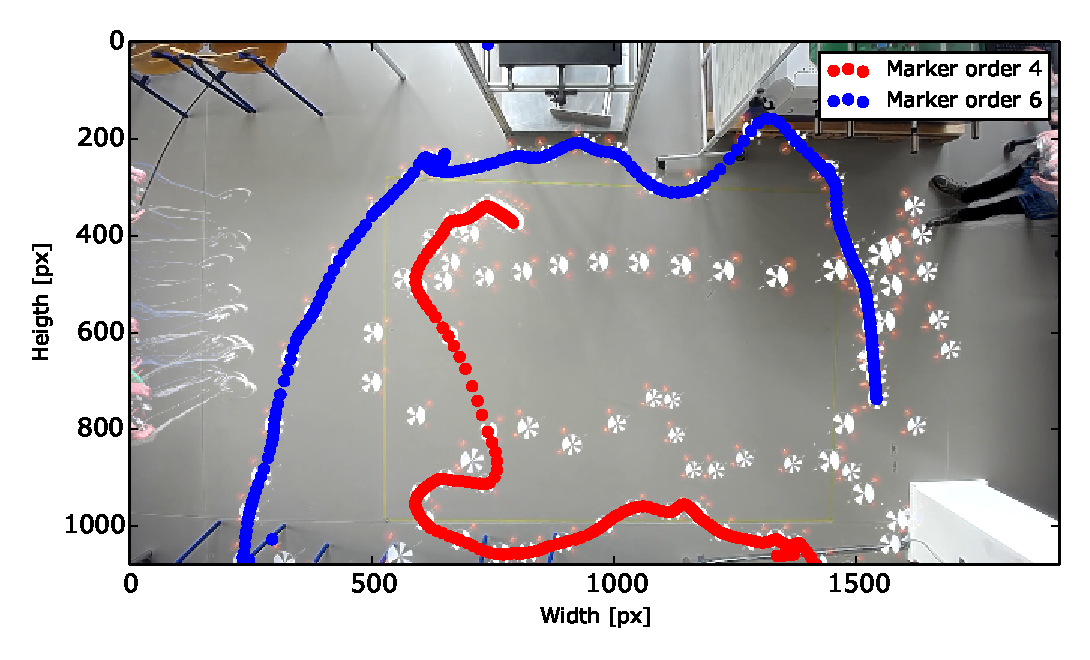
\includegraphics[width=\textwidth]{graphics/markerlocator_compare_raw.eps}
        \caption{Counting pixel match suffers from being unable to find the markers if lost}
        \label{fig:markerlocator_algorihm_native}
    \end{subfigure}
    ~ %add desired spacing between images, e. g. ~, \quad, \qquad, \hfill etc. 
      %(or a blank line to force the subfigure onto a new line)
    \begin{subfigure}[b]{0.3\textwidth}
        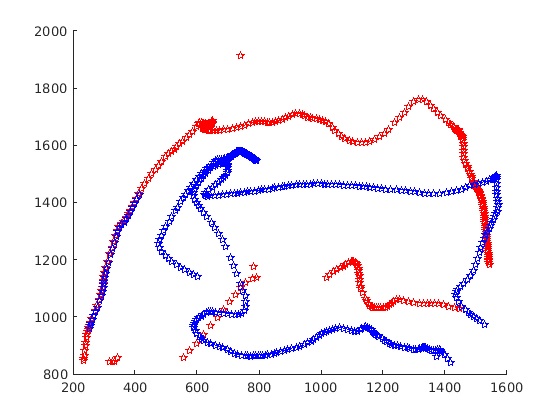
\includegraphics[width=\textwidth]{graphics/markerlocator_ssim.png}
        \caption{SSIM suffers from false positives and a few false negative}
        \label{fig:markerlocator_algorithm_ssim}
    \end{subfigure}
    ~
    \begin{subfigure}[b]{0.3\textwidth}
        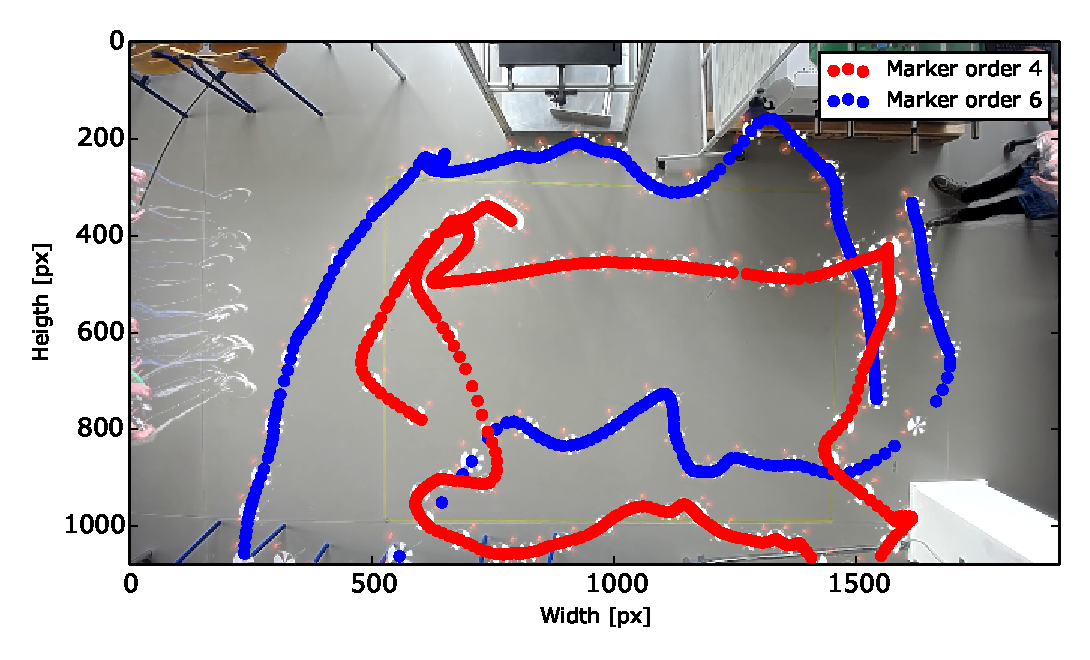
\includegraphics[width=\textwidth]{graphics/markerlocator_match_order.eps}
        \caption{Developed algorithm has no false negative of positive and is able to find the markers if lost}
        \label{fig:markerlocator_algorithm_order_match}
    \end{subfigure}
    \caption{Different approaches to get a quality measure explaining how well the right marker is found.}\label{fig:markerlocator_algorithms}
\end{figure}

Figure \ref{fig:markerlocator_algorihm_native} is a native approach of comparing all pixels in the kernel with the pixels in the found marker. A counter is incremented upon each match and at the end divided by the number of pixels compared in to normalize. A threshold determines weather a marker is found and the next scan should be done in the window of if a full scan is required. The best result is obtained using a threshold of 0.4. If the threshold were lowered false positives started to occur. \\

Figure \ref{fig:markerlocator_algorithm_ssim} uses an algorithm developed to compare similarities in images. 
The details of this algorithm is out of scope the details of this project. The implementation in scipy-image\footnote{\url{http://scikit-image.org/}} was used.
It can seen it performs better than the native approach but a lot of false positive and a few false negative exists. It also suffers from not detecting the markers compared to the native approach. A threshold of 0.3 were used. If the threshold were increased, it would detect less markers. \\

Figure \ref{fig:markerlocator_algorithm_order_match} shows a simple algorithm the author came up with.
If the MarkerLocator is looking for a marker of order 4 and it has detected a marker and its orientation, the algorithm calculates where the location of the arms. It then checks a pixel in each arm and increments a counter if the pixel is black. When it has checked all the arms it compares the counter with the order the MarkerLocator is looking for and returns if they match or not. 
This method does not provide a scalar as output but a binary and thereby has no threshold. However in order to detect if a pixel is black or not, a threshold has been used. The threshold was set to 100 which has shown good results doing tests and flight. \\

During development of quality measures it was noted that if the MarkerLocator does a full search because it cannot find a marker with order 4, it slows down the detection of the marker of order 6. This is because the MarkerLocator is implemented in one process without threading. However this has been solved by splitting up the MarkerLocator in 2 different processes so they run independently of each other. More about this in section  \ref{sec:pc_design} \\

\textbf{Perspective correction} \\
In order to use centimeters as measure of the position of the markers and to correct if the camera is not pointing directly down, the build-in perspective correction in the MarkerLocator were used.
It works by using homography\footcite{janeriksolem2012} to make the transformation from pixels to some chosen unit which in this case is centimeters.
\begin{wrapfigure}{r}{0.5\textwidth}
  \vspace{-20pt}
  \begin{center}
    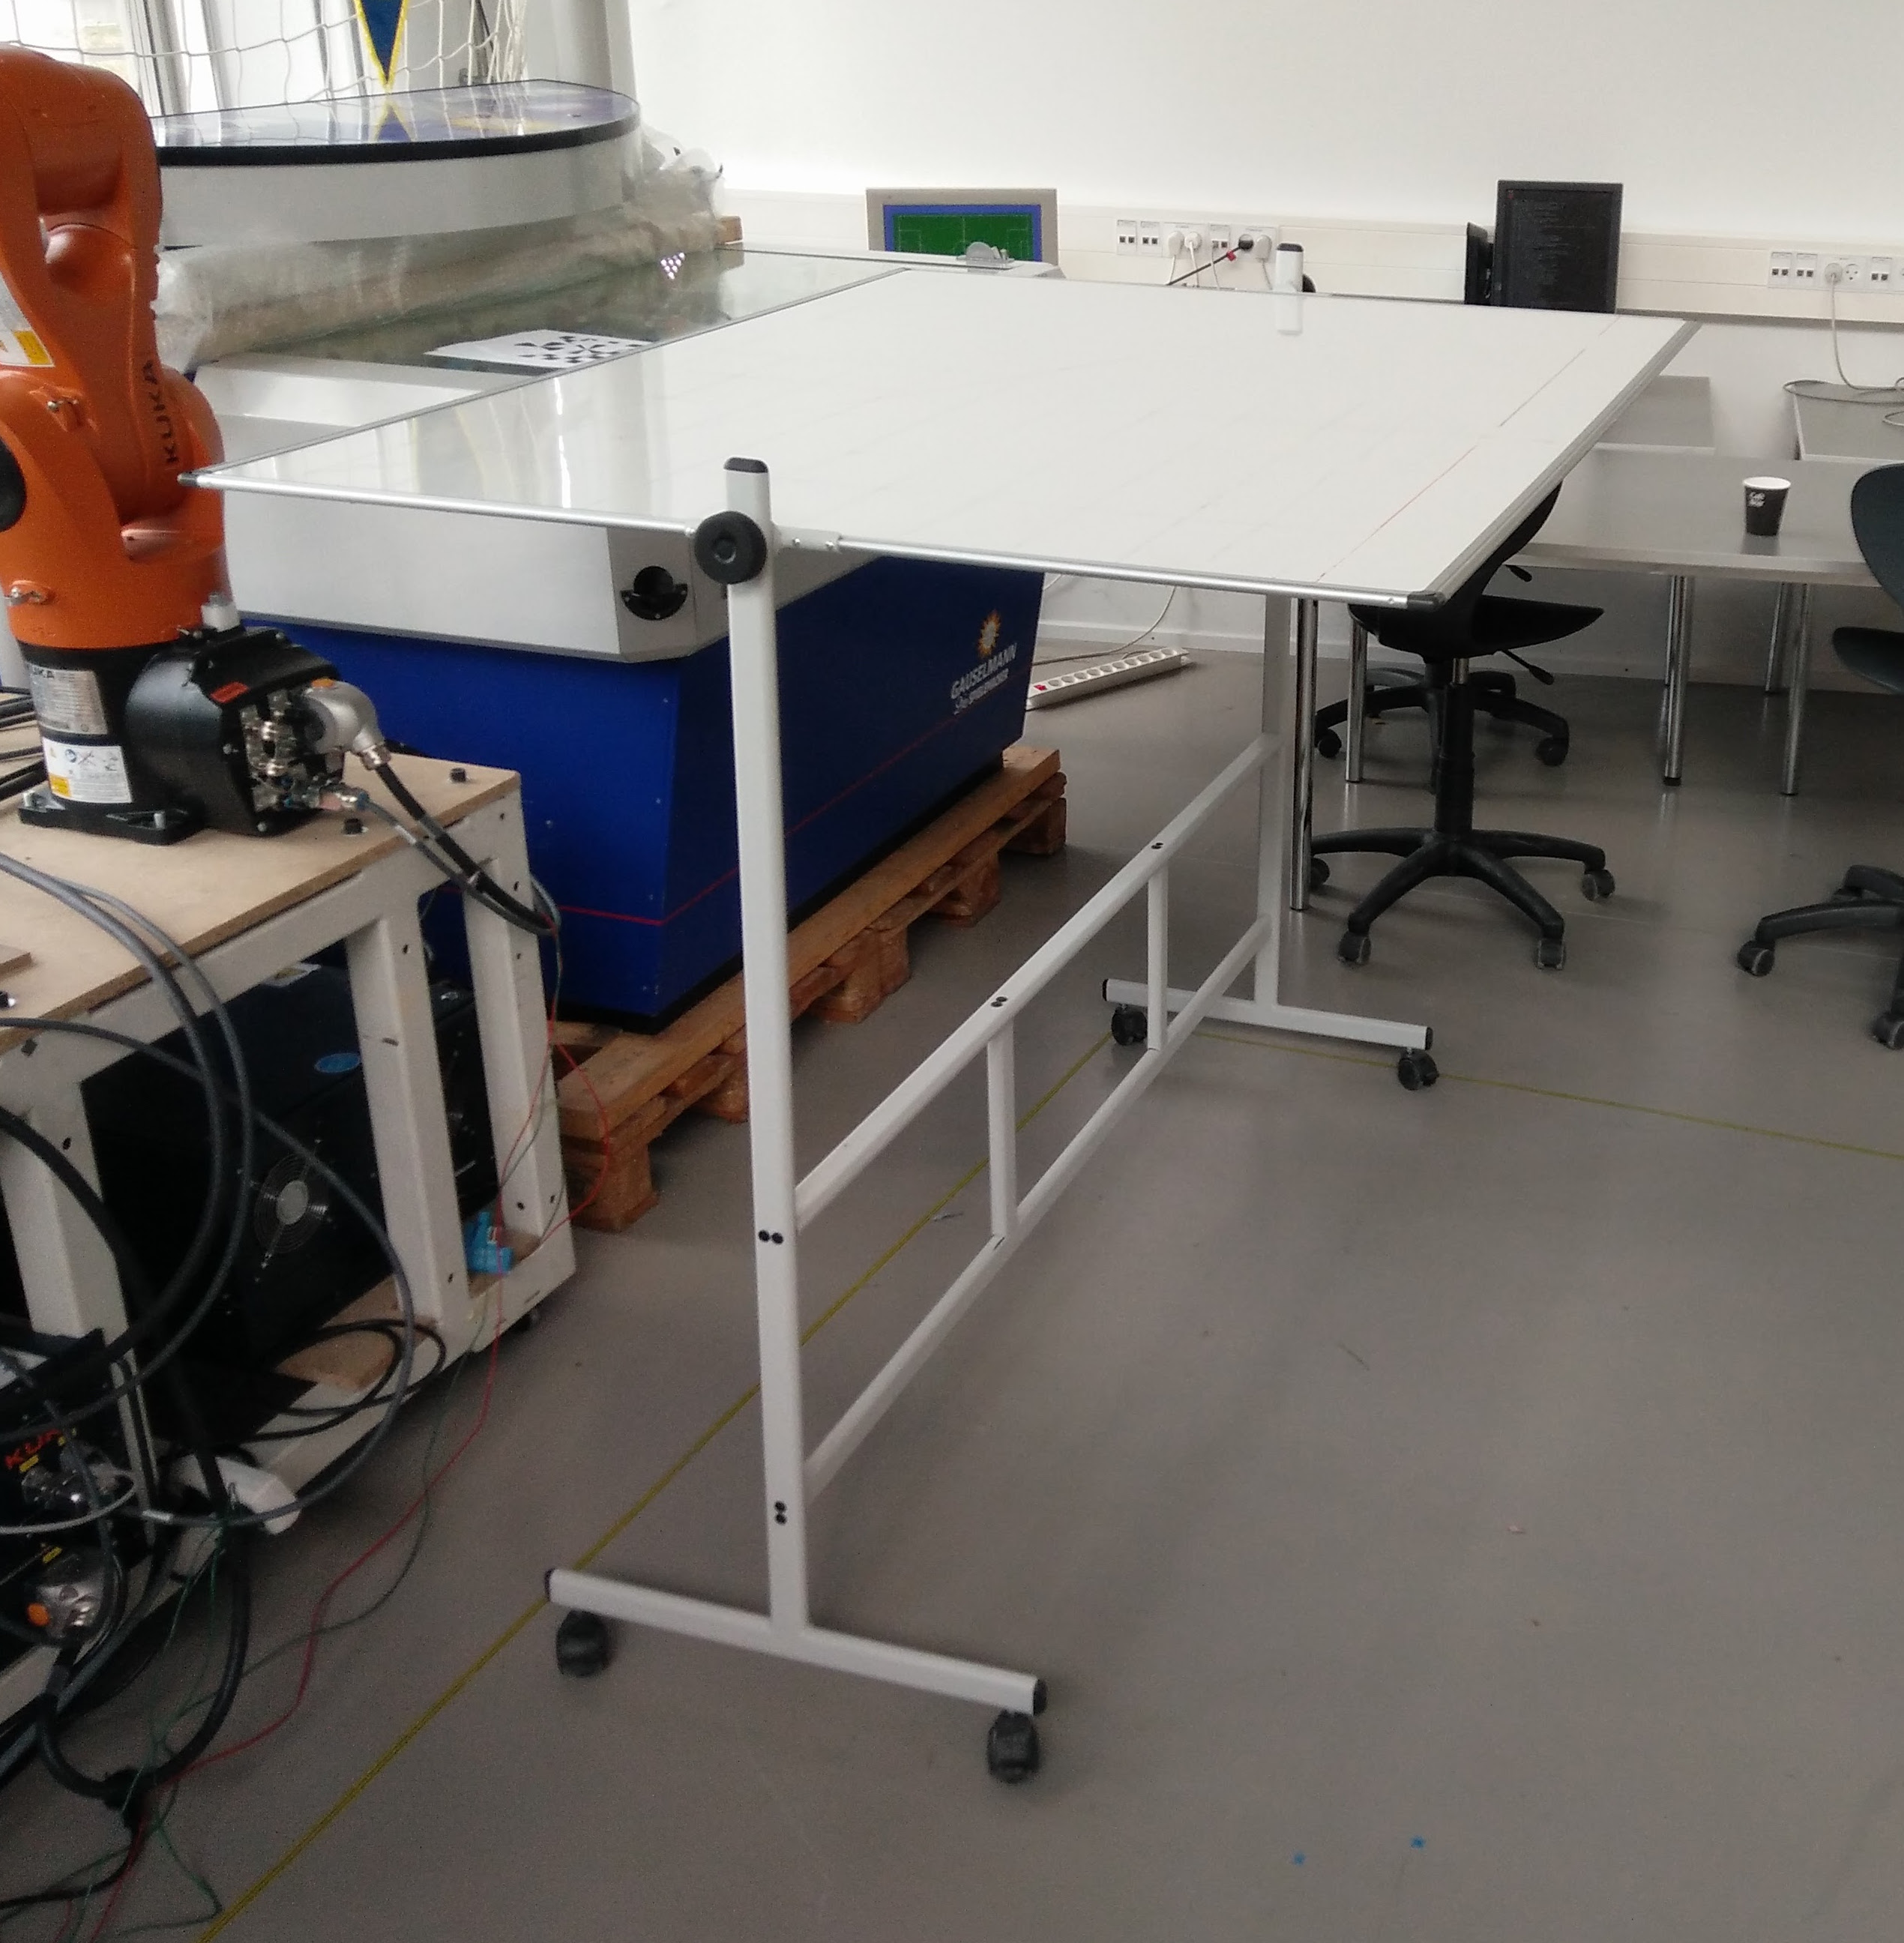
\includegraphics[width=0.48\textwidth]{graphics/whiteboard_tilted.jpg}
  \end{center}
  \vspace{-20pt}
  \caption{Setup used to make 4 points in the flight-height. The four corners of the whiteboard was used and then found in the image. } \label{fig:whiteboard_setup}
  \vspace{-10pt}
\end{wrapfigure}

By creating four markers with known distance to each other at the expected flight height \footnote{Since only 2D positioning is available, a plane where the drone is expected to fly is decided} and find these markers in the frame, it is possible for the perspective corrector to make the transformation.
Figure \ref{fig:whiteboard_setup} shows the setup used. A picture was taken from the ceiling-camera and the four black corners of the whiteboard could be found in the frame. The distance between the black corners in centimeters and the distance in px is given as input to the perspective correcter. The locations of markers is then transformed into the plane made by the whiteboard.


A test was conducted to get the accuracy of the MarkerLocator. Two markers with order 4 and 6 was placed at the expected flight-height and the distance between the two markers was calculated using Pythagoras.\\
The real distance measured by a ruler was 60 cm and and the MarkerLocator gave 59.19 which is an error of 0.81 cm.

Another test was conducted in order to see how stable the MarkerLocator is. 547 position detections was done while the marker was placed steady at the flight height. It shows a mean position in x of -8.1487 with variance of 0, y position with mean -39.5046 and variance 0. \\


It can be concluded that using the MarkerLocator with the improved order detection it is possible to detect two drones without having any false positive/negative. By making a test of the distance between two markers there is an error of 0.81 cm. The MarkerLocator seems stable with a variance of zero. 

newpage

\section{AutoQuad extension board}
\subsection{Introduction}
This secion will go in depth about the extentionboard created as an addon to the AQ M4 board. The extentionboard was developed to act as a bridge between the PC and the CAN-bus using wireless communication.\\
v
The block schematic shown in figure \ref{fig:PCB_block} was created by the auther of the report. It was then given to Carsten Albertsen who created the schematic and did rest of the creation of the PCB.
\\
\subsection{Block schmeatic}
\Mathias{Create schematic appendix}
\Mathias{Add GPS, WIFI, PCB, PC to forkortelses liste}
\Mathias{Thanks to Carsten Albertsen for PCB development}
\begin{figure}[H]
    \center
    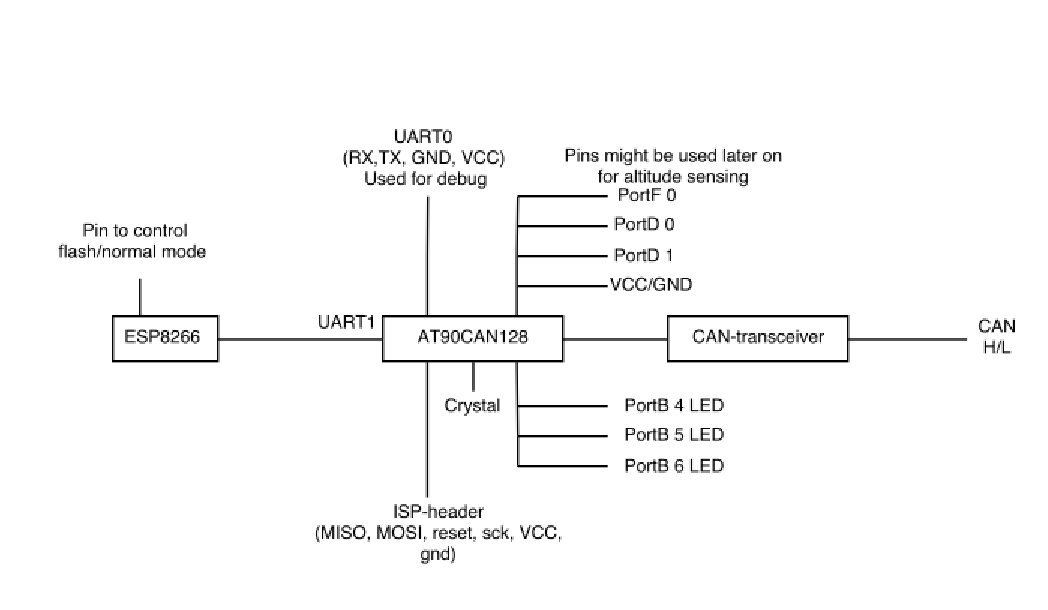
\includegraphics[width=1\textwidth]{graphics/PCB_block_v3.eps}
    \caption{Block schematic of the WIFI-extentionboard developed to AQ M4}
    \label{fig:PCB_block}
\end{figure}

\subsubsection{ATmega}
\subsubsection{Wireless Communication}
An important part of the hardware is the wireless communication used between the PC and the drones.
The wireless communication module has severel requirements it needs to fulfill in order to make the whole system work as expected. A comparison table has been made in table \ref{tab:compare_table_wireless_communication} to find the wireless communication module that is best suited for the task. \\
The following wireless modules where considered and compared.
\begin{itemize}
	\item \textbf{ESP8266}
\end{itemize}

ESP8266 is a generel purpose 32 bit SOC with integrated WIFI 802.11 b/g/n support and buildin TCP/IP stack. It can be setup its own access point or it can connect to an existing wireless network.
It runs at 80MHz and can be flashed with a custom firmware. 
The SOC is sold as modules with different pinouts and features such as extra flash memory \footnote{\url{https://www.olimex.com/Products/IoT/MOD-WIFI-ESP8266/open-source-hardware}} and different antennas.
The chip has been on the marked for about two years and costs approximately 7\$. 
It has been widely used in DIY-projects due to its low price and because it requires a minimum of network knowledge to get up and running.\footnote{\url{http://www.esp8266.com/} - 43.000 posts in forum} When the SOC is shipped, it comes with a preloaded firmware which either accepts AT commands or LUA scripting depending on the version of the module. These simple programming interfaces makes it quick and easy to interface the cheap. \\
This leads to a large community where most of the problems have been found and solved already. Arduino has been ported to ESP8266 which makes it even easier to get it up and running. Their official Arduino GitHub has 2125 commits on their master branch at the time of writing\footnote{\url{https://github.com/esp8266/Arduino}} \\

\begin{itemize}
	\item \textbf{EMW3165}
\end{itemize}
EMW3165 is a SOC much like the ESP8266 supporting 802.11 b/g/n WIFI with buildin TCP/IP stack. As with ESP8266 it supports setting up an access point aswell as connecting to an existing network. It has a Cortex-M4 $\mu$C which run at 100MHz. 
It supports custom firmware and can be aswell be bought as different modules with different pinouts and antennas.
It differentiates itself from the ESP8266 by its higher frequency its 5 volts compatible pins \footnote{\url{https://hackadaycom.files.wordpress.com/2015/07/emw3165.pdf}} which makes it easier to connect other hardware which run 5 volt without the need of a logic level shifter. It has been on the marked for only one year and costs approximately 9\$. Since it is a newer board than ESP8266 it has not been used in the same number of applications and thereby has a smaller community behind\footnote{\url{http://www.emw3165.com/} - 200 posts in forum }. Their most active GitHub has 147 commits on their master branch at the time of writing\footnote{\url{https://github.com/SmartArduino/WiFiMCU}}.

\begin{itemize}
	\item \textbf{nRF51822}
\end{itemize}
nRF51822 is also a SOC, but it is using Bluetooth instead of WIFI. The nRF51822 $\mu$C is implementing BLE which is a power efficient way of sending and receiving data. The chip supports broadcasting which could be used in this project. The $\mu$C can be bought as a standalone component or mounted on modules as the two other $\mu$Cs. Different modules offers different types of antenna connectors or buildin antenna on the PCB. It has not been possible to find an Arduino ported firmware that supports this $\mu$C. To write a firmware for the $\mu$C it has to be done using Nordic Semiconductor's proprietary SDK. 


\begin{itemize}
	\item \textbf{XBee}
\end{itemize}
XBee is a module that implements the Zbee standard. The Xbee modules work as a wireless serial connection. The Xbee modules supports mesh networking which means the modules by themself figure out which module is closest and makes the connection. This idea makes sense in this application since there will be multiple drones and one computer. If one drone gets too far from the PC, it can just connect to one of the other drones closer to the PC.\\
The Xbee solution is ready to use and requires a minimum of programming to get up and running. The modules also support GPIO for digital in and output and analog input.

\Mathias{ '\'footmotemark til at referere til samme fodnote flere gange}
\begin{table}[H]
	\centering
	\begin{tabular}{@{}|l|l|l|l|l|l|l|l|@{}}
		\toprule
		\textbf{Product} & \textbf{Size} & \textbf{Weight} & \textbf{Price} & \textbf{Documentation} &  \textbf{Range}  & \textbf{Score} \\ \midrule
		ESP8266   &  24x16mm\footnote{\url{https://www.mikrocontroller.net/attachment/243558/fcc\_11.pdf}} \hfill\{7\} & 1.5g\footnote{Measured by author on chemistry weight} \hfill\{8\} &   7.5\$\footnote{\url{http://www.seeedstudio.com/depot/ESP8266-based-WiFi-module-SPI-supported-p-2486.html}}    &   Great community \hfill\{9\}  &    ?    &                		\\ \midrule
		EMW3165   &  32x16mm\footnote{\url{https://hackadaycom.files.wordpress.com/2015/07/emw3165.pdf}} \hfill\{6\}  & 5g\footnote{\url{http://www.seeedstudio.com/depot/EMW3165-CortexM4-based-WiFi-SoC-Module-p-2488.html}} \hfill\{2\} &  9\$\footnote{\url{http://www.seeedstudio.com/depot/EMW3165-CortexM4-based-WiFi-SoC-Module-p-2488.html}}   &  Less available  \hfill\{3\}	        &    ?    &                		\\ \midrule
		nRF51822  &  18x10mm\footnote{\url{http://www.fanstel.com/Product/bluenor.html}} \hfill\{8\}  & 3g\footnote{\url{http://www.seeedstudio.com/depot/MDBT40P\%C2\%A0\%C2\%A0nRF51822\%C2\%A0based\%C2\%A0BLE\%C2\%A0module-p-2503.html}} \hfill\{0\}  &  7.5\$  & Ok documented\hfill\{2\} 	        &   30 M\footnote{\url{https://dl.dropboxusercontent.com/u/54939426/Fanstel_BT600.pdf}}  \hfill\{9\}     &                		\\ \midrule
		XBee      &  24.38x27.61mm \footnote{\url{http://www.digi.com/products/xbee-rf-solutions/modules/xbee-802-15-4\#specifications}} \{3\} & 3g \footnote{\url{http://www.digi.com/products/xbee-rf-solutions/modules/xbee-802-15-4\#specifications}} \hfill\{4\} &   25\$\footnote{\url{https://www.sparkfun.com/products/11215}}    &  Lots of DIY   \hfill\{9\}      &            91 M\footnote{\url{https://www.sparkfun.com/pages/xbee_guide}}  \hfill\{9\}  &                    \\ \bottomrule
	\end{tabular}
	\caption{Comparisontable used to compare different wireless 		communication modules}
	\label{tab:compare_table_wireless_communication}
\end{table}
\Mathias{vægt på ESP til 3 gram med link - det er hvad der er oplyst. Efterfølgende skrive at det er vejet til 1.51 gram(hen mod slutningen)}
The products compared in \ref{tab:compare_table_wireless_communication} are chosen to have approximately same specs. Onboard antenna, breakout for easy pin access.

\subsubsection{Pins}
A few pins where made available through solder pads for easy access if needed later on.

The following pins where available as solder pads:
\begin{itemize}
	\item PortF 0 - Alternative function as ADC, channel 0
	\item PortD 0 - Alternative function as interrupt, INT0
	\item PortD 1 - Alternative function as interrupt, INT1
\end{itemize}
In case the onboard baromter isn't accurate enough, an alternative distance could be used to measure the drones altitude with respect to the ground.
PortF0 has been made available since some distance sensors give output as an analogue value. 
An example of such sensor is an Infrared proximity sensor.\footnote{\url{http://www.sharpsma.com/webfm\_send/1208}} \\
As an alternative type of distance sensor, a ultrasoinc could be used such as HCSR04.
As output it gives a binary output with high-time proportional with the distance.\footnote{\url{http://www.micropik.com/PDF/HCSR04.pdf}}.
To detect the high-time, one of PortD1/0 would be useful. \\

Which type of sensor suits best as a distance sensor to provice altitude information to the drone is ouf of the scope of this report. The PCB has just been made ready to different types of sensors.

\subsubsection{Debug/ISP}
In the final schematic UART0 and ISP pins where combined in one pinheader for easy access through one cable. \Mathias{Refer to image of board}
To program the AtMega the ISP pins where required to be easy accessable. 
UART0 was made accessable to be used as debug and programming of the ESP8266 board.
The plan was to setup the AtMega as UART passthrough from UART0 to UART1.
Due to a mistake\footnote{The wrong pair of MISO/MOSI pins where made available in the ISP-header. The correct pair of MISO/MOSI is also RXD0/TXD0 as alternative function} in the final schematic, both UART0 and UART1 where made accessable trough the ISP/debug header. 
This ended up making it easier to program the ESP8266-board without using the AtMega as UART passthrough.

ESP noteS:
 - GPIO15 = bootmode, low for ...
 - GPIO0 = flash mode
 
 
 https://zoetrope.io/tech-blog/esp8266-bootloader-modes-and-gpio-state-startup

\newpage

\section{AutoQuad M4 firmware}
\textit{Since AutoQuad only supports proving GPS coordinates through a serial port\footnote{Seen by inspection of the schematic to the M4-board done by the supervisor} another way had to be found and implemented.
Sending GPS coordinates through the serial port would require the onboard GPS to be unmounted which seems like a bad solution. The CAN bus was chosen since it is already implemented in AutoQuad. However AutoQuad supports sensor inputs through CAN, GPS was not supported and there by had to be implemented.}

In order to send GPS coordinates to AQ a way in had to be found. A solution would be to unmount the onboard GPS, however that removes the functionality of the M4 board to fly normally without external hardware eg. A RPI. Since AutoQuad gets its coordinates from the onboard ublox M8Q \footnote{\url{http://autoquad.org/wiki/wiki/m4-microcontroller/m4-gps-antenna-options/}} using ublox's ubx protocol, everything sent by eg. a RPI had to be encoded as ubx.
Instead of making hardware changes to the M4 it was decided to use the already supported CAN-bus interface. The M4 board already uses the CAN-bus to send velocities to each of the ESC's on an EduQuad drone. AutoQuad default supports sending some sensor values using the CAN-bus, however GPS coordinates, DOPs and accuracies was not implemented. The only implementation was to receive the battery voltage and current usage and log it to an MicroSD-card.
AutoQuads CAN protocol is described, implemented and tested in section \ref{sec:somewhere}.

When all CAN-nodes has successfully registered, different node-initializing functions run.
First a summary run which sends the number and types of the nodes to QGroundStation. \footnote{Graphical userinterface which provices generel information about the drone such as battery, attitude but also waypoint functionalities}.
It can thus be validated by the pilot that all the ESC's and CAN-sensors are detected.
After the summary, a CAN-sensor initialization happens. The initialization of each CAN-sensor happens which is to send CAN\_CMD\_TELEM\_* described in section \ref{sec:somewhere} but more important also to create a callback.
The callback will then be attached to the CAN-type which in this case is CAN-sensor\footnote{CAN-types are described in section \ref{sec:somewhere}} so when AutoQuad receives a sensor reading the callback will be invoked.\\

Default the callback fills in the sensorvalue in an array so the sensor value can be used in another task. The canID \footnote{Described in section \ref{sec:somewhere}} is then used as index so the task needing the sensorvalue knows where to look since it knows which sensorsvalue it needs. Code \ref{code:callback} shows the callback\footnote{\url{https://github.com/bn999/autoquad/blob/master/onboard/canSensors.c}}
\begin{lstlisting}[language = c, caption = Callback invoked when a CAN-sensorvalue is received. It stores the value in an array indexed by canId, label=code:callback]
void canSensorsReceiveTelem(uint8_t canId, uint8_t doc, void *data) {
    canSensorsData.values[canId] = *(float *)data;

	/* Reception time of the message stored as well */
}
\end{lstlisting}
The callback is fairly simple and does not save the doc\footnote{Described in section \ref{sec:somewhere}} which is needed in order to tell which value the CAN-GPS sensor is sending.\\

All of the CAN-GPS packet handling has been implemented in the callback function. A prettier solution might have been to create a task and use a semaphore to signal when there is a new GPS-packet available. Due to lack of time implementing everything was done in the callback.

Code \ref{code:psudo_parse_can_gps} shows a pseudo code of how the GPS-packets is handled. In section \ref{sec:somewhere} the CAN-GPS packets can be seen.

\begin{lstlisting}[language = Matlab, caption = Modified callback invoked when a sensor-value is received. Shows how doc is used to tell which GPS\-packet is received and when height is received the flags are set, label=code:psudo_parse_can_gps]
canSensorsReceiveTelem(canId, doc, *data) {
	if doc == CAN_DOC_LAT then
		canData.latitude = data
		
	if doc == CAN_DOC_LON then
		canData.longitude = data
		
	if doc == CAN_DOC_DOP then
		canData.xDOP = data[x]
		..
	if doc == CAN_DOC_ACC then
		canData.satellites = data[0]
		canData.fix = data[1]
		canData.xAcc = data[x]
		..
		canData.heading = data[n-1]
		
	if doc == CAN_DOC_VEL then
		gpsData.velx = data[x]
		..		
	if doc == CAN_DOC_ALT then
		gpsDatat.height = data
		if gpsData.fix == 1 and gpsData.satellites >= 8 then
			gpsUpdatetime = now()
			setFlag (gpsData.gpsPosFlag)
			setFlag (gpsData.gpsVelFlag)
		else:
			debug_to_QGroundStation
}
\end{lstlisting}

The \textit{data} pointer given as parameter to the callback is of void pointer. Some pointer gymnastics is done in order to get the right elements from the CAN-packet. If the received CAN-packet is of 8*1 bytes, the void pointer is casted to an uint8\_t pointer so each byte can be retrieved by using the casted pointer as an array. \\

When the flags are set, the task updating the UKF will run \footnote{\url{https://github.com/bn999/autoquad/blob/master/onboard/run.c\#L110} last visited 23 maj}.
Code \ref{code:ukf_update} shows a snippet from the task updating the UKF when the position or velocity flag is set.
\begin{lstlisting}[language = Matlab, caption = Snippet of run.c as psudeocode which updates the UKF when position flag or velocity flag is set, label=code:ukf_update]
if IsFlagSet(gpsData.gpsPosFlag) == yes then
	    navUkfGpsPosUpdate(gpsData.lastPosUpdate, gpsData.lat, gpsData.lon, gpsData.height, ....);
	    ClearFlag(gpsData.gpsPosFlag);
	    
else if IsFlagSet(gpsData.gpsVelFlag) == yes then
	    navUkfGpsVelUpdate(gpsData.lastVelUpdate, gpsData.velN, gpsData.velE, ....);
	    ClearFlag(gpsData.gpsVelFlag);
\end{lstlisting}

\section{AutoQuad extension board firmware}
\textit{In this chapter the development of the firmwares running on the extension board is described. Different types of schedulers for the At90CAN128 is discussed and a scheduler is chosen and developed with the required functionality. The communication between PC and M4 is further described. At the end of each section a test is conduced in order to show if the code works as expected }
\subsection{Scheduler}
\textit{This capter concerns only the Atmega.  The ESP module will be descriped in section \ref{sec:esp_firmware}} \\
In order to have a timing on the At90CAN128 a scheduler was chosen and implemented.
The list below shows 3 different types of scheduler that was considered.
\begin{itemize}
	\item Real-time Operating System(RTOS) provides strict timing but at the cost of overhead. A RTOS runs task in a "parallel" environment. Each task runs in a loop and the RTOS scheduler will do context switching when needed. Using a RTOS requires mutexes and semaphores to protect shared resources which increases the complexity and amount of overhead
	\item Super-Loop provides no timing at all, but process data as fast as possible. It does not do any context switching and does not require mutexes or semaphores and  and thereby takes no overhead.
	\item Run-To-Complete(RTCS) scheduler is a mix of the two other schedulers. It works by waiting for a tick generated by a hardware timer and then starts executing all tasks from the beginning. The order of the task matters if there is dependency between the tasks but also to make sure the task requiring the most precise timing is at the beginning of the list of the tasks. All tasks have to be finished executing before the next tick is giving in order to avoid timing is ruined.
\end{itemize}
The RTCS was chosen since it provides timing without the overhead created when doing context-switching and the need of mutex and semaphores. It further reduces the code-complexity.\\

It was decided to implement the code in tasks to make a low coupling between the functionalities. This makes it easier to maintain and expand later of if needed. The task diagram shown in figure \ref{fig:task_diagram_atmega} shows the tasks and how they do intertask communication.


\begin{figure}[H]
    \center
    \includegraphics[width=0.9\textwidth]{graphics/task_diagram.png}
  \label{fig:task_diagram_atmega}
  \caption{Tasks diagram showing overview of the running tasks on the At90Can128}
\end{figure}



\subsubsection*{Test of RTCS timing}
In order to test the timing of the scheduler, a led\_task was written. The task can be seen in code \ref{code:test_scheduler}
\begin{lstlisting}[language = c, caption = RTCS task used in timing test, label=code:test_scheduler]
void is_alive_task(uint8_t my_state){

	// Write to UART0
	UDR0 = my_state+'0';

	switch(my_state){
	case 0:
		INT_LED_ON_GREEN;
		INT_LED_OFF_RED;
		INT_LED_OFF_BLUE;
	    set_state( 1 );
		break;
	case 1:
		INT_LED_OFF_GREEN;
		INT_LED_ON_RED;
		INT_LED_OFF_BLUE;
	    set_state( 2 );
		break;
	case 2:
		INT_LED_OFF_GREEN;
		INT_LED_OFF_RED;
		INT_LED_ON_BLUE;

		// Set next state
	    set_state( 0 );
		break;
	}
	// Wait one second
	wait( 1000 );
}
\end{lstlisting}

The test was done by writing the current state of the task to UART0.\\ A python script were made that measures the time between each character received. The script can be seen in code \ref{code:test_rtcs_python}.
\begin{lstlisting}[language = python, caption = Python code used to measure time between received byte, label=code:test_rtcs_python]
#!/usr/bin/python
import serial
import time

ser = serial.Serial( port='/dev/ttyUSB0', baudrate=57600 )

t = time.time()
while True:
    for char in ser.read(1):
        print time.time() - t, ","
        t = time.time()

ser.close()
\end{lstlisting}
The output of the script were redirected to a file. After receiving 700 bytes the standard deviation and mean was calculated using matlab.
The mean is 1.0089 sec with a standard deviation of 0.0042 sec.

Part of the variance is caused by the inaccuracy of the timing on the PC running the python code. If a more accurate measure was needed, a scope could be attached to the $\mu$C's GPIO. Each time the scheduler enters the task the GPIO should be set high, and when it exists the GPIO should be set low. The scopes at SDU is capable of telling the variance of the off signal. \\
It can be concluded that the scheduler performs well.
\newpage

\subsection{Queues}
\subsection*{Test of CAN, queues}
In order to test CAN and queues, a task was written. The purpose of the task was to receive a CAN-message if any available from the queue and send the ID and data from the CAN message to a PC using UART.
The task used can be seen in code \ref{code:test_can_uart_task}.


\begin{lstlisting}[language = c, caption = Task used to test CAN, label=code:test_can_uart_task]
CAN_frame frame;
if(QueueReceive(&Queue_CAN_Rx, &frame)) {
	char ch;
	/* ID out uart0 */
	for(int i = 3; i >=0; i--){
		ch = ((frame.id >> i*8) & 0x000000FF);
		QueueSend(&Queue_Uart0_Tx,&ch);
	}
	/* ID end*/

	/* MSG out uart0 */
	for(int i = (frame.dlc-1); i >=0; i--){
		ch = ((frame.msg >> i*8) & 0x00000000000000FF);
		QueueSend(&Queue_Uart0_Tx,&ch);
	}
	/* MSG end */

	/* End of line */
	ch = '\r';
	QueueSend(&Queue_Uart0_Tx,&ch);
	ch = '\n';
	QueueSend(&Queue_Uart0_Tx,&ch);
}
\end{lstlisting}
The command used to send CAN-messages can be seen in code \ref{code:bash_send_can}.

\begin{lstlisting}[language = bash, caption = Task used to test CAN, label=code:bash_send_can]
while true; do sleep 1; print $(date); cansend can0  1DEADBEF#FEDCBA9876543210; done
\end{lstlisting}
The command sends a CAN-message using a connected PEAK-CAN adapter. It sends a message each second and prints out the date to make it clear when it is sending a message.\\ \textit{1deadbef} is the 29 bit ID and \textit{fedcba9876543210} is the 64 bit data. \\


The command used to show the received HEX values can be seen in code \ref{code:xxd}

\begin{lstlisting}[language = bash, caption = Command used to get UART messages, label=code:xxd]
cat /dev/ttyUSB0 | xxd -c 14 
\end{lstlisting}
Cat reads from /dev/ttyUSB0 and pipes its output to xxd where it is shown in HEX.\\ -c is number of columns which is 14 due to 4 ID bytes, 8 data bytes and 2 as newline.\\

The result can be seen in figure \ref{fig:can_recv_output}.
\begin{figure}[H]
    \center
    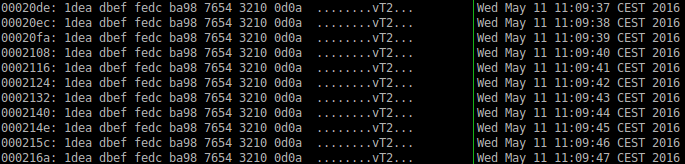
\includegraphics[width=1\textwidth]{graphics/xdd_can_test.png}
  \label{fig:boat1}
  \caption{Left shows output from command \ref{code:xxd} and right shows command \ref{code:bash_send_can}}
\end{figure}
It can be seen that the received ID and data is \textit{1deadbef} and \textit{fedcba9876543210} respectively.\\
\textit{0d0a} is \textbackslash r and \textbackslash n respectively.



\newpage
%\subsection{Tasks}
%\input{tasks}
%\newpage

%\subsection{Wireless communication}
%\subsubsection*{Communication flow}
\begin{table}[H]
\centering

\begin{tabularx}{0.75\textwidth}{@{}|X|X|X|X|X|X|@{}}
\toprule
Content & Lat    & Lon    & Height & DOP   & CRC-16  \\ \midrule
Datatype    & double & double & float  & float & uint16\_t \\ \midrule
Bytes    & 31:24  & 23:16   & 15:8    & 7:4 & 3:0 \\ \bottomrule
\end{tabularx}
\Mathias{Ændre 0:3 til 0:1 da en uint16\_t kun tager 2 bytes og ikke 4}
\caption{Message sent from PC to ESP8266}
\label{my-label}
\end{table}


bstract.tex


\newpage



\newpage


  can0  00000000   [0] 
  can0  01C00000   [8]  EF BE AD DE 03 09 00 00
  can0  0E000041   [6]  EF BE AD DE 00 00
  can0  14CD0042   [2]  00 08
  can0  14CC0043   [2]  0A 00



seq tæller op så rate/value bliver acknowledged
  can0  00000000   [0] 
  can0  01C00000   [8]  EF BE AD DE 03 09 00 00
  can0  0E000041   [6]  EF BE AD DE 00 00
  can0  14CD0042   [2]  00 08
  can0  00400002   [8]  00 00 00 00 00 00 00 00
  can0  14CC0043   [2]  0A 00
  can0  00400003   [8]  00 00 00 00 00 00 00 00


\newpage